\PassOptionsToClass{onlytextwidth}{beamer}
%%
% This is an Overleaf template for presentations
% using the TUM Corporate Desing https://www.tum.de/cd
%
% For further details on how to use the template, take a look at our
% GitLab repository and browse through our test documents
% https://gitlab.lrz.de/latex4ei/tum-templates.
%
% The tumbeamer class is based on the beamer class.
% If you need further customization please consult the beamer class guide
% https://ctan.org/pkg/beamer.
% Additional class options are passed down to the base class.
%
% If you encounter any bugs or undesired behaviour, please raise an issue
% in our GitLab repository
% https://gitlab.lrz.de/latex4ei/tum-templates/issues
% and provide a description and minimal working example of your problem.
%%

%% ================================== base ================================== %%
\documentclass[
	german,            % define the document language (english, german)
	aspectratio=169,    % define the aspect ratio (169, 43)
	% handout=2on1,       % create handout with multiple slides (2on1, 4on1)
	% partpage=false,     % insert page at beginning of parts (true, false)
	% sectionpage=true,   % insert page at beginning of sections (true, false)
]{tumbeamer}

\usepackage{booktabs}
\usepackage{enumerate}
\usepackage{float}

% fvextra must be loaded before csquotes (minted pulls it in later)
\usepackage{fvextra}

%% ================================ language ================================ %%
\usepackage{babel}[ngerman]
\usepackage{csquotes}[autostyle]
\usepackage[useregional]{datetime2}
\usepackage{pmboxdraw}

%% ================================== math ================================== %%
\usepackage{amsmath}
\usepackage{amssymb}
\usepackage{ifthen}

%% ================================ graphics ================================ %%
\usepackage{graphicx}
\usepackage{xcolor}
\usepackage{pifont}
\usepackage{url}
\usepackage{hyperref}

\graphicspath{ {./resources/} }

%% ================================== tikz ================================== %%
\usepackage{pgf}
\usepackage{tikz}
\usepackage{pgfplots}
\usepackage{tikz-timing}
\usepackage{circuitikz}
\usepackage{karnaugh-map}

\usetikzlibrary{arrows, arrows.meta, backgrounds, positioning,
	shapes, shapes.geometric, shapes.symbols,
	patterns, patterns.meta,
	matrix, fit, calc,
	decorations.pathreplacing,
	tikzmark, chains,
	overlay-beamer-styles,
	automata}

% requires circuitikz >= 1.1.0
% for distros with older distributions, install TeX Live manually
% instead of using your package manager
% see: https://tug.org/texlive/quickinstall.html
\ctikzset{logic ports=european}

%% ============================= code listings ============================= %%
\usepackage[cache=true]{minted}
\usepackage{listings}

\usemintedstyle{borland}
\setminted{
	fontsize=\small,
	frame=none,
	breaklines=true,
}

%% ============================ colors & styling ============================ %%
\renewcommand{\thempfootnote}{\arabic{mpfootnote}}
\setbeamercolor{footnote}{fg=black}
\setbeamercolor{footnote mark}{fg=black}

%% ============================= custom macros ============================= %%
% https://tex.stackexchange.com/a/7045
\newcommand*\circled[1]{\tikz[baseline=(char.base)]{
		\node[shape=circle,draw,inner sep=2pt, font=\scriptsize] (char) {#1};}}

\newcommand*\colorcirc[1]{\tikz[baseline=(char.base)]{
		\node[shape=circle,fill=#1,inner sep=2pt] {};}}

\newcommand{\n}[1]{\overline{#1}}

%% ================================ metadata ================================ %%
\author{Niklas Ladurner}
\institute{\theChairName\\\theDepartmentName\\\theUniversityName}

\footline{\insertauthor~|~\insertshorttitle~|~\insertshortdate}

\TUMbeamersetup{
	title page = TUM tower,         % style of the title page
	part page = TUM toc,            % style of part pages
	section page = TUM toc,         % style of section pages
	content page = TUM more space,  % style of normal content pages
	tower scale = 1.0,              % scaling factor of TUM tower (if used)
	headline = TUM threeliner,      % which variation of headline to use
	footline = TUM default,         % which variation of footline to use
	% configure on which pages headlines and footlines should be printed
	headline on = {title page},
	footline on = {every page, title page=false},
}

% available frame styles for title page, part page, and section page:
% TUM default, TUM tower, TUM centered,
% TUM blue default, TUM blue tower, TUM blue centered,
% TUM shaded default, TUM shaded tower, TUM shaded centered,
% TUM flags
%
% additional frame styles for part page and section page:
% TUM toc
%
% available frame styles for content pages:
% TUM default, TUM more space
%
% available headline options:
% TUM empty, TUM oneliner, TUM twoliner, TUM threeliner, TUM logothreeliner
%
% available footline options:
% TUM empty, TUM default, TUM infoline


\title{Übung 09: Automaten \\und
	Multi-Cycle-Prozessor}
\subtitle{Einführung in die Rechnerarchitektur}
\date{\DTMdisplaydate{2024}{12}{13}{-1}}

\begin{document}

\maketitle

\begin{frame}[c, fragile]{}{}
	\begin{center}
		\LARGE  Keine Garantie für die Richtigkeit der Tutorfolien.

		\Large Bei Unklarheiten/Unstimmigkeiten haben VL/ZÜ-Folien recht!
	\end{center}
\end{frame}

\begin{frame}[fragile, c]{Endliche Automaten}{}
	\begin{itemize}
		\item Repräsentiert Funktion einer sequentiellen Schaltung (sequentiell: zustandsabhängig)
		\item als Diagramm: Zustände $\rightarrow$ Kreise, Übergänge $\rightarrow$ Kanten, Bedingungen $\rightarrow$ Kantenbeschriftungen
		\item als 6-Tupel $(I, O, S, s_0, \delta, \lambda)$:
		      \begin{itemize}
			      \item $I$: Menge möglicher Eingaben
			      \item $O$: Menge möglicher Ausgaben
			      \item $S$: Zustandsmenge
			      \item $s_0$: Startzustand
			      \item $\delta:  S\times I\rightarrow S$: Zustandsübergangsfunktion
			      \item $\lambda: S\rightarrow O$ (Moore), $\lambda: S\times I\rightarrow O$ (Mealy): Ausgabefunktion
		      \end{itemize}
	\end{itemize}
\end{frame}

\begin{frame}[fragile, c]{Endliche Automaten: Beispiele}{}
	\begin{columns}[c]
		\begin{column}{0.5\textwidth}
			\begin{center}
				\textbf{Moore-Automat}\\
				{\scriptsize Ausgabe abhängig von aktuellem Zustand}\\
				\resizebox{!}{0.65\textheight}{
					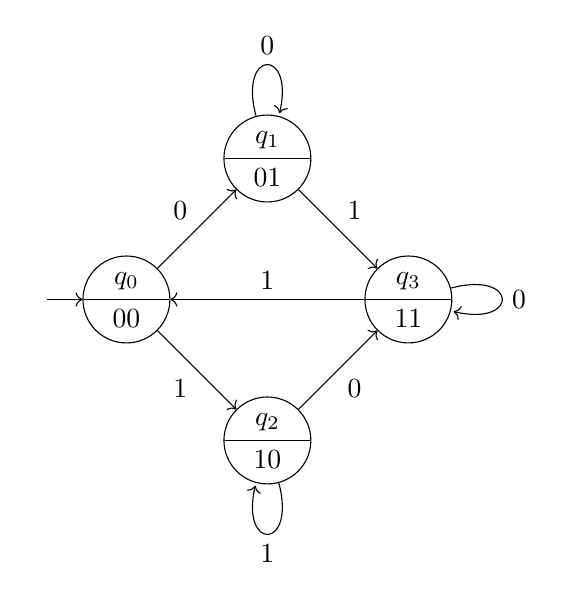
\begin{tikzpicture}[initial text=]
						\node[state with output, initial] (q0) {$q_0$  \nodepart{lower} $00$};
						\node[state with output] (q1) [above right=of q0] {$q_1$  \nodepart{lower} $01$};
						\node[state with output] (q2) [below right=of q0] {$q_2$  \nodepart{lower} $10$};
						\node[state with output] (q3)  [below right=of q1] {$q_3$  \nodepart{lower} $11$};

						\path[->, every node/.style={execute at begin node=$, execute at end node=$}]
						(q0) edge node [above left]  {0} (q1)
						edge node [below left]  {1} (q2)
						(q1) edge node [above right] {1} (q3)
						edge [loop above] node {0} ()
						(q2) edge node [below right] {0} (q3)
						edge [loop below] node {1} ()
						(q3) edge [loop right] node {0} ()
						(q3) edge node [above] {1} (q0);
					\end{tikzpicture}
				}
			\end{center}
		\end{column}
		\begin{column}{0.5\textwidth}
			\begin{center}
				\textbf{Mealy-Automat}\\
				{\scriptsize Ausgabe abhängig von aktuellem Zustand + Eingabe}\\
				\resizebox{!}{0.65\textheight}{
					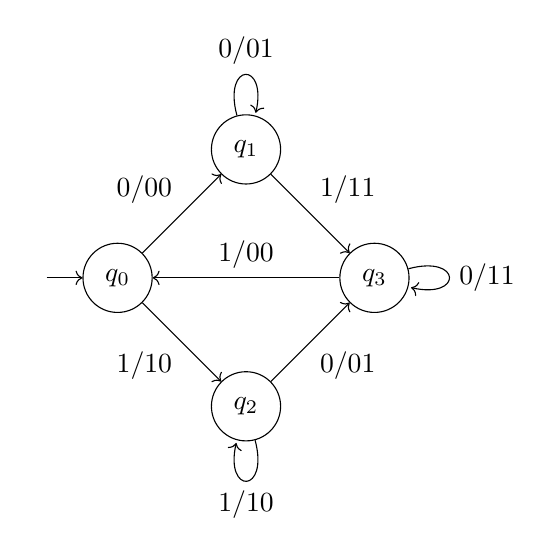
\begin{tikzpicture}[initial text=]
						\node[state, initial] (q0) {$q_0$  \nodepart{lower} $00$};
						\node[state] (q1) [above right=of q0] {$q_1$};
						\node[state] (q2) [below right=of q0] {$q_2$};
						\node[state] (q3)  [below right=of q1] {$q_3$};

						\path[->, every node/.style={execute at begin node=$, execute at end node=$}]
						(q0) edge node [above left]  {0/00} (q1)
						edge node [below left]  {1/10} (q2)
						(q1) edge node [above right] {1/11} (q3)
						edge [loop above] node {0/01} ()
						(q2) edge node [below right] {0/01} (q3)
						edge [loop below] node {1/10} ()
						(q3) edge [loop right] node {0/11} ()
						(q3) edge node [above] {1/00} (q0);
					\end{tikzpicture}
				}
			\end{center}
		\end{column}
	\end{columns}
	\begin{center}
		{\scriptsize $I=\{0, 1\}$, $O=\{00, 01, 10, 11\}$, $S=\{q_0, q_1, q_2, q_3\}, \delta, \lambda$ (abh. vom Typen)}
	\end{center}
\end{frame}

\begin{frame}[fragile, c]{Endliche Automaten: Realisierung}{}
	\begin{columns}[c]
		\begin{column}{0.5\textwidth}
			\begin{itemize}
				\item One-Hot-Kodierung: Genau 1 FF ist auf 1 (aktueller Zustand), einfach aber verschwenderisch
				\item Binärkodierung: FFs zusammen bilden Binärzahl des aktuellen Zustands, spart FFs aber komplexer
				\item Mikroprogrammierte Steuerwerke: Nur ein Speicherbaustein, enthält vollständigen Automaten. Eingaben werden als Adressen interpretiert, sehr flexibel.
			\end{itemize}
		\end{column}
		\begin{column}{0.5\textwidth}
			\begin{table}[]
				\begin{tabular}{c|c|c}
					Zustand & One-Hot & Binär \\ \hline
					$S_0$   & $0001$  & $00$  \\
					$S_1$   & $0010$  & $01$  \\
					$S_2$   & $0100$  & $10$  \\
					$S_3$   & $1000$  & $11$
				\end{tabular}
			\end{table}
		\end{column}
	\end{columns}
\end{frame}

\begin{frame}[c]{Adressmodifizierendes \\\vspace{-0.75cm}mikroprogrammiertes Steuerwerk}{}
	\resizebox{\textwidth}{!}{
		\begin{circuitikz}
			\tikzset{
				every node/.style={minimum width=2.5cm, minimum height=0.7cm, text height=1.5ex, text depth=0ex},
				mat/.style={ampersand replacement=\&, row sep=-\pgflinewidth, column sep=0.25cm, nodes={draw}},
				addr/.style={draw=none, align=right, minimum width=0.5cm, text width=0.25cm},
				code/.style={anchor=west, draw=none, align=left, font=\ttfamily, text width=7.6cm, xshift=1cm},
				mux1/.style={muxdemux, muxdemux def={NL=4, NR=1, NT=1, NB=0}, anchor=center, xscale=-0.5, yscale=0.4},
				iopt/.style={anchor=center, minimum width=1cm}
			}

			\matrix[matrix of nodes, mat] (romContent){
				\node[addr] {}; \& Folgeadresse \& Bedingung \& Steuersignale \\
				\node[addr] {$00$:}; \& $10$ \& $01$ \& $0$                   \\
				\node[addr] {$01$:}; \& $01$ \& $10$ \& $1$                   \\
				\node[addr] {$10$:}; \& $00$ \& $11$ \& $0$                   \\
				\node[addr] {$11$:}; \& $00$ \& $00$ \& $1$                   \\
			};

			\node[code] at (romContent-2-4.east) {if a then goto 10 else goto 01;};
			\node[code] at (romContent-3-4.east) {while b;};
			\node[code] at (romContent-4-4.east) {if c then goto 00 else goto 11;};
			\node[code] at (romContent-5-4.east) {goto 00;};

			\node[anchor=south] at (romContent.north) (romHeader) {\textbf{ROM}};
			\node[draw, fit=(romContent) (romHeader)] (romContainer) {};


			\node[iopt, yshift=4cm, xshift=5.5cm]  at (romContent-1-4.east) (condIopt) {Bedingung};
			\node[mux1, below=of condIopt] (condMux) {};

			\draw (condIopt.south) to[bmultiwire] (condMux.tpin 1);
			\draw (condMux.lpin 1) -- ++(1,0) node[iopt, right] {1};
			\draw (condMux.lpin 2) -- ++(1,0) node[iopt, right] {a};
			\draw (condMux.lpin 3) -- ++(1,0) node[iopt, right] {b};
			\draw (condMux.lpin 4) -- ++(1,0) node[iopt, right] {c};

			\draw (condMux.rpin 1) -- ++(-1, 0) node[left, text width=3cm, text depth=2cm, text height=2cm, anchor=east, align=center] {Adresse + 1 oder Folgeadresse?};
		\end{circuitikz}
	}
\end{frame}


\begin{frame}[c, fragile]{RISC-V Multi-Cycle-Prozessor}{}
	\begin{itemize}
		\item Aufteilung einer Instruktion in mehrere Schritte
		\item kürzere kritische Pfade in den einzelnen Teilschritten $\rightarrow$ höhere Taktfrequenz möglich
		\item allerdings benötigt eine Instruktion jetzt auch mehrere Taktzyklen!
		\item komplexeres Steuerwerk, da Zustandsautomat umgesetzt werden muss
	\end{itemize}
	\begin{center}
		in der Praxis haben sich Multi-Cycle-Prozessoren nicht durchgesetzt!
	\end{center}
\end{frame}

\begin{frame}[c]{RISC-V Multi-Cycle-Prozessor: Schaltbild}{}
	\begin{center}
		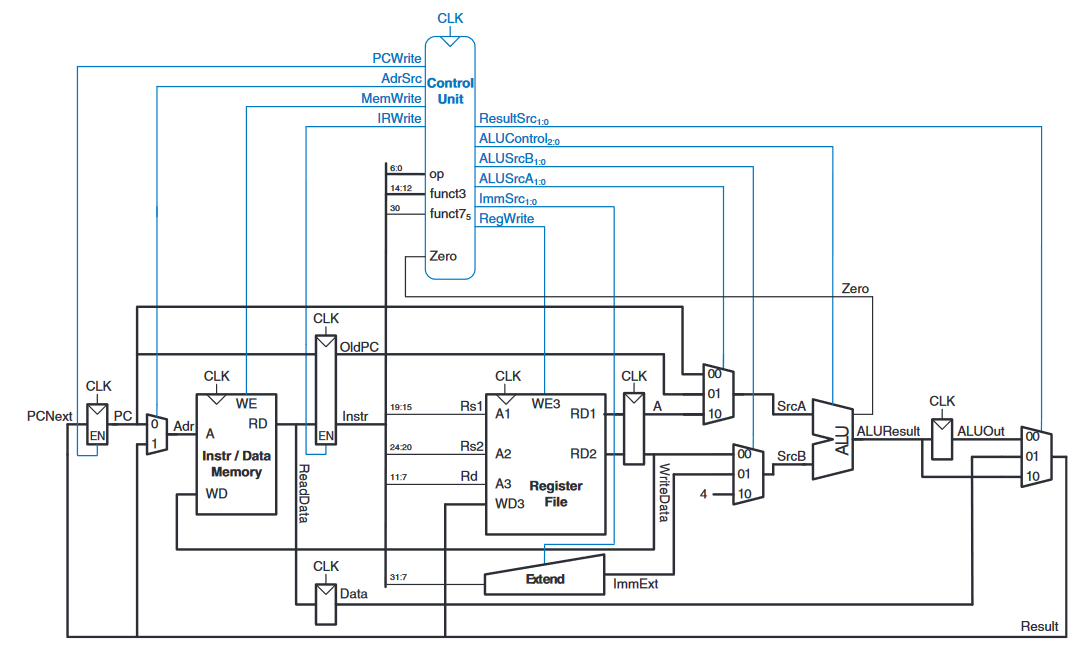
\includegraphics[width=0.75\textwidth]{w09_multicycle.png}
	\end{center}
	\centering
	\tiny (Quelle: Vorlesungsmaterialien ERA)
\end{frame}

\begin{frame}[c]{RISC-V Multi-Cycle-Prozessor: Zustandsautomat}{}
	\begin{center}
		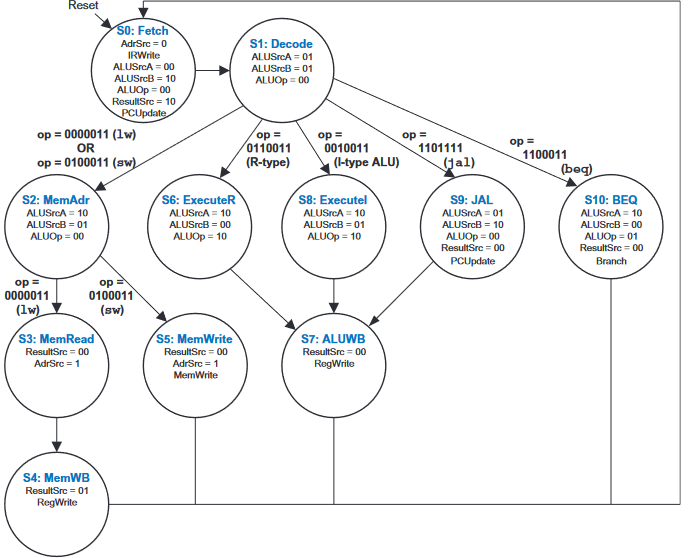
\includegraphics[width=0.6\textwidth]{w09_multicycle_states.png}
	\end{center}
	\centering
\end{frame}

\begin{frame}[c, fragile]{Artemis-Hausaufgaben}{}
	\begin{itemize}
		\item \enquote{H09 --- Sequenzielles Steuerwerk} bis 05.01.2025 23:59 Uhr
		\item Implementierung des Steuerwerks des Multi-Cycle-Prozessors
		\item \texttt{StateUpdate.dig} kann durchaus umfangreich werden
	\end{itemize}
\end{frame}

\begin{frame}[c, fragile]{Links}{}
	\begin{itemize}
		\item Zulip: \href{https://zulip.in.tum.de/#narrow/stream/2661-ERA-Tutorium---Do-1600-1}{\enquote{ERA Tutorium - Do-1600-1}}
		      bzw. \href{https://zulip.in.tum.de/#narrow/stream/2675-ERA-Tutorium---Fr-1500-2 }{\enquote{ERA Tutorium - Fr-1500-2}}
		\item \href{https://www.moodle.tum.de/course/view.php?id=100633}{ERA-Moodle-Kurs}
		\item \href{https://artemis.in.tum.de/courses/401}{ERA-Artemis-Kurs}
		\item \href{https://courses.edx.org/assets/courseware/v1/f06a2dc0c856f60ec0711e9f5e1c98cf/asset-v1:HarveyMuddX+ENGR85B+1T2023+type@asset+block/FinalReferences.pdf}{Prozessor-Assets (kein offizielles Material!)}
	\end{itemize}
\end{frame}

\maketitle

\end{document}
